\section{Error Propagation} \label{sec:error_propagation}

\subsection{Law of propagation of uncertainties method}
\subsection{MonteCarlo method}
\subsection{Example: SAR Wind Retrieval}
\label{sec: OSWV}

The \gls{traceability} diagram for OSWV retrieval is presented for an algorithm that uses a Bayesian approach.
The a-posteriori conditional probability density function (pdf) of the retrieved ocean surface wind vector (OSWV) $\mathbf{u}$ can be modeled as reported in Equation \ref{eq: AP pdf}, which is a generalization of the approach proposed in \cite{PortabellaJGRO2002}.

\begin{equation}
	\mathrm{pdf}_{\mathbf{u}|\sigma_{0},f_{dc},\lambda_{C},\mathbf{u_{B}}} \propto \mathrm{pdf}_{\mathbf{u}|\mathbf{u_{B}}} \mathrm{pdf}_{\sigma_{0}|\mathbf{u}} \mathrm{pdf}_{\lambda_{C}|U} \mathrm{pdf}_{f_{w}|\mathbf{u},f_{dc}}
	\label{eq: AP pdf}
\end{equation}

In Equation \ref{eq: Bayes}, $\sigma_{0}$ is the measured Normalized Radar Cross Section (NRCS), $\mathrm{pdf}_{\mathbf{u}|\mathbf{u_{B}}}$ is the conditional pdf of 
$\mathbf{u}$, known the a-priori (background) OSWV $\mathbf{u_{B}}$, $\mathrm{pdf}_{\sigma_{0}|\mathbf{u}}$ is the conditional pdf of the NRCS prediction model, 
$\mathrm{pdf}_{\lambda_{C}|U}$ is the conditional pdf of the azimuth wavelength cut-off ($\lambda_{C}$) prediction model, known the wind speed ($U$), and 
$\mathrm{pdf}_{f_{w}|\mathbf{u}}$ is the conditional pdf of the  prediction model of the Doppler Centroid Anomaly (DCA) wind component ($f_{w}$), known DCA 
($f_{dc}$). $\mathbf{u_{B}}$ is provided by Numerical Weather Prediction (NWP) models, such as those from the European Centre for Medium-Range Weather Predictions 
(ECMWF). \\
The optimal solution corresponds to the value of $\mathbf{u}$ that maximizes the a-posteriori conditional pdf. \\
Assuming that all pdfs are Gaussian, this is equivalent to minimize the cost function reported in Equation \ref{eq: Bayes}

\begin{eqnarray}
	J = \frac{\bar{\sigma}_{0}-\mathrm{GMF}_{\sigma_{0}}(\mathbf{u},\theta,\nu,pol)}{\Delta \bar{\sigma}_{0}}+\frac{\mathbf{u}-\mathbf{u_{B}}}{\Delta \mathbf{u_{B}}}+ \nonumber \\
	\frac{\lambda_{C}-\mathrm{GMF}_{\lambda_{C}}(U,\theta,\nu,pol)}{\Delta \lambda_{C}}+\frac{f_{w}-\mathrm{GMF}_{f_{w}}(\mathbf{u},\theta,\nu,pol,f_{dc})}{\Delta f_{w}}
	\label{eq: Bayes}
\end{eqnarray}

where $\theta$ is the incidence angle, $\nu$ is the signal carrier frequency, $pol$ is the polarization of the signal. and $\mathrm{GMF}$ stands for Geophysical Model Function, which is the prediction model. As the name suggests, a GMF is an empirical forward model relating the geophysical parameter domain to the observable domain. In this notation, the symbol $\bar{\sigma}_{0}$ states that NRCS is averaged over a given area, typically of 1-2 km per side. This is required to mitigate wave modulation and reduce the speckle \cite{MigliaccioJOE2007}. \\
For a C-band SAR such as Sentinel-1, CMOD7 \cite{StoffelenJSTARS2017} is used as the NRCS prediction model. The explicit formulation of CMOD7 is reported in Equation \ref{eq: CMOD7} for the sake of completeness,

\begin{eqnarray}
	z = A_{0}(U,\theta) \left[ A_{1}(U, \theta) \cos(\phi)+A_{2}(U, \theta) \cos(2\phi) \right] \\
	z = \sigma_{0}^{0.625} \nonumber
	\label{eq: CMOD7}
\end{eqnarray}

with $z$ the transformed backscattering coefficient, $U$ the wind speed, $\phi$ the relative wind direction with respect to the antenna looking angle, and $A_{i}, \ \forall i \in \left\{ 0,1,2 \right\}$, the fitting coefficients derived empirically. \\
In the first term of Equation \ref{eq: Bayes}, $\Delta \bar{\sigma}_{0}$ is the uncertainty of $\bar{\sigma}_{0}$, which we may model as the sum of the contributions from measurement uncertainty ($\Delta \bar{\sigma}_{0}^{M}$) and prediction model ($\Delta \bar{\sigma}_{0}^{S}$).
The same contribution model can be hypothesized for $\Delta \lambda_{C}=\Delta \lambda_{C}^{M}+\Delta \lambda_{C}^{S}$ and $\Delta f_{w}=\Delta f_{w}^{M}+\Delta f_{w}^{S}$, which represent the uncertainties of $\lambda_{C}$ and $f_{w}$, respectively. Finally, $\Delta \mathbf{u_{B}}$ is the uncertainty of $\mathbf{u_{B}}$. \\ 
In the following treatment, the symbols $\epsilon$ and $\Delta$ have the same meaning. We will use $\epsilon$ to indicate the error source and $\Delta$ for the terms explicitly stated in Equation \ref{eq: Bayes}. Therefore, the notation $\epsilon(\Delta \bar{\sigma}_{0})$ stands for the error source in the estimate of the uncertainty of $\bar{\sigma}_{0}$. \\ 
The analytical propagation of errors in $\mathbf{u}$ is quite complex and not easily quantifiable using an analytical approach; therefore, the error sources will be discussed separately for each term of Equation \ref{eq: Bayes}, and a graphical explanation will be preferred instead of an analytical treatment of the problem. \\
Focusing on the first term of Equation \ref{eq: Bayes}, the following error sources will contribute to the uncertainty of $J$:
\begin{itemize}
	\item $\epsilon(\bar{\sigma}_{0})$: uncertainty of measured and simulated $\bar{\sigma}_{0}$ values, namely $\epsilon(\bar{\sigma}_{0}^{M})$ and $\epsilon(\bar{\sigma}_{0}^{S})$, respectively. The first term depends on the instrument radiometric error, while the second depends on the accuracy of the prediction model (see next point);
	\item uncertainty of $\mathrm{CMOD7}$. The model is considered error-free. From a formal point of view, its deviation from reality is accounted for in the uncertainty of the coefficients $A_{i}$ ($\epsilon(A_{i})$);
	\item $\epsilon(\theta)$: uncertainty of the incidence angle. This can be due to errors in the model used to compute $\theta$ and to antenna pointing errors. This error source is estimated to be very small;
	\item $\epsilon(\Delta \bar{\sigma}_{0})$: uncertainty of $\Delta \bar{\sigma}_{0}$ estimate. As said before, this quantity has two contributions, namely $\epsilon(\Delta \bar{\sigma}_{0}^{M})$ and $\epsilon(\Delta \bar{\sigma}_{0}^{S})$;
	\item $\epsilon(pol)$: uncertainty introduced by eventual signal leaking due to channel cross-talk. In C-band, this error source is supposed to be small. This may not be the case of other spectral bands, such as L-band, due to signal interactions with the ionosphere; 
\end{itemize}

In the second term of Equation \ref{eq: Bayes}, there are two sources of uncertainty:
\begin{itemize}
	\item $\epsilon(\mathbf{u_{B}})$: uncertainty of the background term;
	\item $\epsilon(\Delta \mathbf{u_{B}})$: uncertainty of the error source indicated in the previous point;
\end{itemize}
In the third term, the additional error sources that were not discussed before are listed below:
\begin{itemize}
	\item $\epsilon(\lambda_{C})$: uncertainty of the azimuth wavelength cut-off estimate;
	\item $\epsilon(\Delta \lambda_{C})$: uncertainty of the previous error source;
	\item uncertainty of the prediction model ($\mathrm{GMF}_{\lambda_{C}}$). As shown in \cite{CorcioneTGRS2019,GriecoIJRS2016}, the dependency of $\lambda_{C}$ on $U$ is supposed to be linear in fully developed sea states, as written in Equation \ref{eq: az cutoff}:
	\begin{equation}
		\lambda_{C}=a_{0}+a_{1}U
		\label{eq: az cutoff}
	\end{equation}
	The deviation of the model from reality is accounted for in the uncertainty of the coefficients $a_{i}$ ($\epsilon(a_{i})$);
\end{itemize}

In the last term, the additional error sources are:
\begin{itemize}
	\item $\epsilon(f_{dc})$: uncertainty of DCA;
	\item $\epsilon(f_{elec})$: uncertainty due to antenna electronic mis-pointing;
	\item $\epsilon(f_{sca})$: uncertainty due to scalloping;
	\item $\epsilon(f_{att})$: uncertainty due to satellite attitude variations;
	\item $\epsilon(f_{osc})$: uncertainty of the estimate of the DCA ocean surface current component;
	\item $\epsilon(f_{ss})$: uncertainty of the estimate of the DCA sea state component;
\end{itemize}

Figure \ref{fig: OSWV diag} shows the uncertainty \gls{traceability} diagram for the OSWV algorithm discussed in this section.

\begin{figure}[h]
	\centering
	\newcommand\ys{1.cm}
	\newcommand\xs{2.cm}
%\fontsize{8}{9}\selectfont
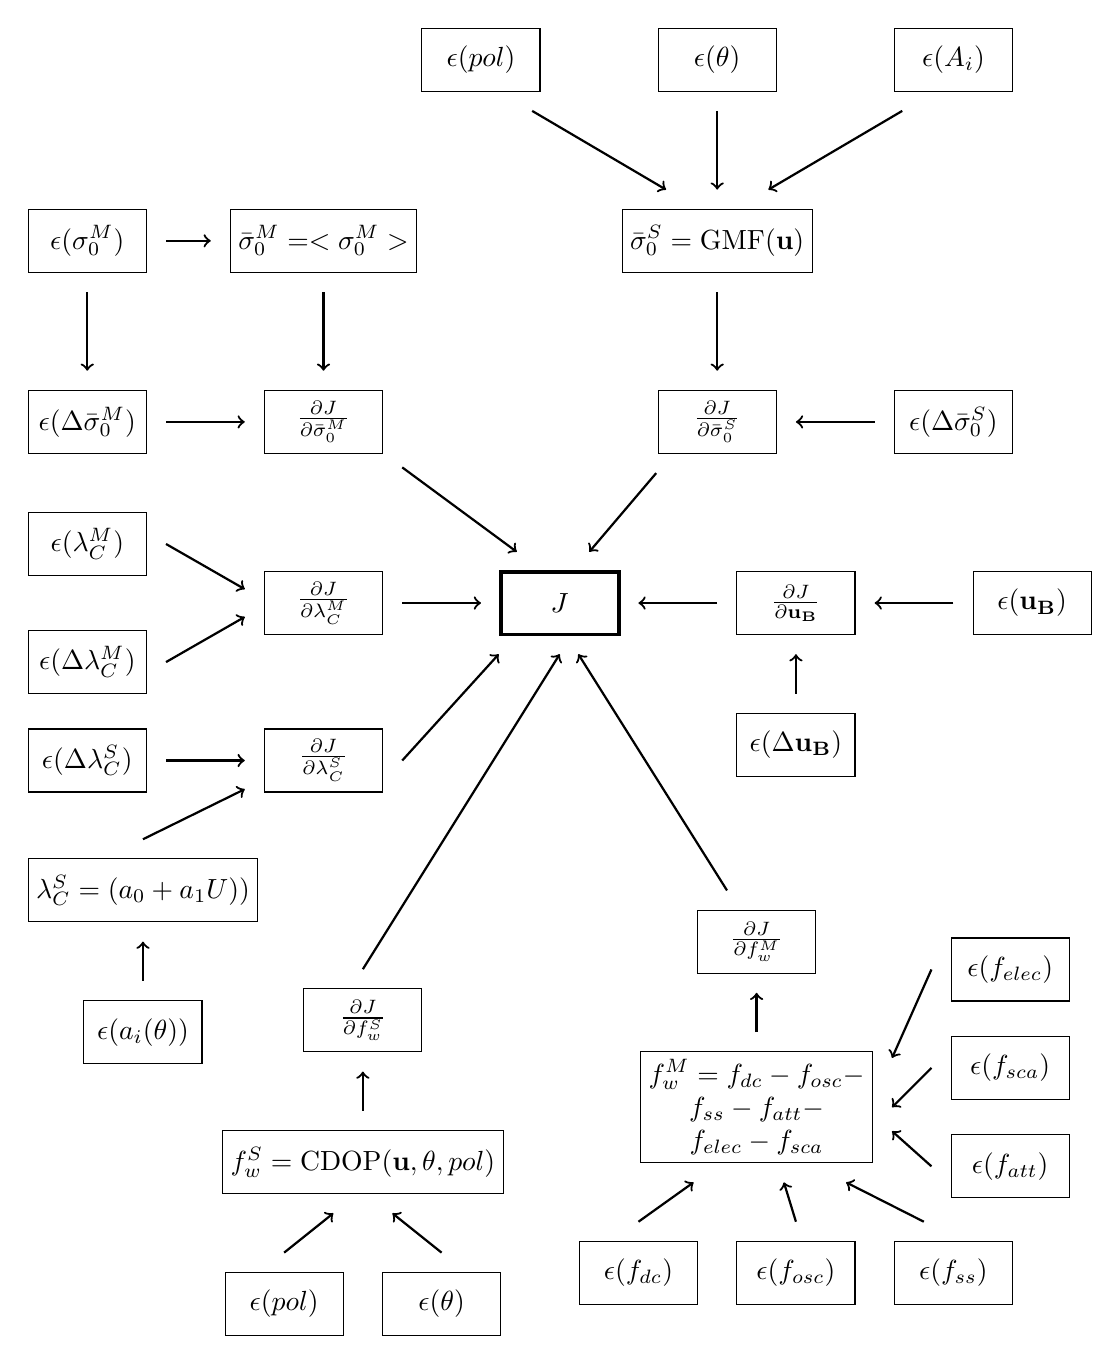
\begin{tikzpicture}[myarrow/.style={single arrow,single arrow head extend=.1cm,anchor=west,minimum height=.8cm,minimum width=.1cm},
	myrectangle/.style={rectangle,draw=black,text=black,inner sep=.1cm, outer sep=.25cm, minimum width=1.5cm, minimum height=.8cm}],
% ------------------------------------------------------------------------------------
% ------------------ Cost function block ---------------------------------------------
% ------------------------------------------------------------------------------------
	\node(J)[myrectangle,line width=.5mm,align=center,anchor=east] at (0.cm, 0.cm) {$J$};
% ------------------------------------------------------------------------------------
% ------------------ Measured sigma0 block -------------------------------------------
% ------------------------------------------------------------------------------------
	\node(dJds0)[myrectangle,align=center,anchor=south] at ([xshift=-1.5*\xs,yshift=\ys]J.north) {$\frac{\partial J}{\partial \bar{\sigma}_{0}^{M}}$};
	\node(uDs0M)[myrectangle,align=center,anchor=east] at ([xshift=-\xs]dJds0) {$\epsilon(\Delta \bar{\sigma}_{0}^{M})$};
	\node(uas0)[myrectangle,align=center,anchor=south] at ([yshift=\ys]dJds0.north) {$\bar{\sigma}_{0}^{M}=<\sigma_{0}^{M}>$};
	\node(us0)[myrectangle,align=center,anchor=south] at ([yshift=\ys]uDs0M.north) {$\epsilon(\sigma_{0}^{M})$};
	\path [black, thick, ->] (uDs0M.0) edge node {} (dJds0.180);
	\path [black, thick, ->] (uas0.270) edge node {} (dJds0.90);
	\path [black, thick, ->] (dJds0.330) edge node {} (J.130);
	\path [black, thick, ->] (us0.0) edge node {} (uas0.180);
	\path [black, thick, ->] (us0.270) edge node {} (uDs0M.90);
% ------------------------------------------------------------------------------------
% ------------------ Simulated sigma0 block ------------------------------------------
% ------------------------------------------------------------------------------------
	\node(dJdGMF)[myrectangle,align=center,anchor=south] at ([xshift=\xs,yshift=\ys]J.north) {$\frac{\partial J}{\partial \bar{\sigma}_{0}^{S}}$};
	\node(uDs0S)[myrectangle,align=center,anchor=west] at ([xshift=\xs]dJdGMF) {$\epsilon(\Delta \bar{\sigma}_{0}^{S})$};
	\node(GMF)[myrectangle,align=center,anchor=south] at ([yshift=\ys]dJdGMF.north) {$\bar{\sigma}_{0}^{S}=\mathrm{GMF}(\mathbf{u})$};
	\node(utheta)[myrectangle,align=center,anchor=south] at ([yshift=\ys]GMF.north) {$\epsilon(\theta)$};
	\node(uA)[myrectangle,align=center,anchor=west] at ([xshift=.5*\xs]utheta.east) {$\epsilon(A_{i})$};
	\node(upol)[myrectangle,align=center,anchor=east] at ([xshift=-.5*\xs]utheta.west) {$\epsilon(pol)$};
	\path [black, thick, ->] (upol.315) edge node {} (GMF.135);
	\path [black, thick, ->] (GMF.270) edge node {} (dJdGMF.90);
	\path [black, thick, ->] (utheta.270) edge node {} (GMF.90);
	\path [black, thick, ->] (uA.225) edge node {} (GMF.45);
	\path [black, thick, ->] (uDs0S.180) edge node {} (dJdGMF.0);
	\path [black, thick, ->] (dJdGMF.220) edge node {} (J.60);
% ------------------------------------------------------------------------------------
% ------------------ Background block ------------------------------------------------
% ------------------------------------------------------------------------------------
	\node(dJduB)[myrectangle,align=center,anchor=west] at ([xshift=.5*\xs]J.east) {$\frac{\partial J}{\partial \mathbf{u_{B}}}$};
	\node(uuB)[myrectangle,align=center,anchor=west] at ([xshift=0.5*\xs]dJduB.east) {$\epsilon(\mathbf{u_{B}})$};
	\node(uDuB)[myrectangle,align=center,anchor=north] at ([yshift=-0.5*\ys]dJduB.south) {$\epsilon(\Delta \mathbf{u_{B}})$};
	\path [black, thick, ->] (dJduB.180) edge node {} (J.0);
	\path [black, thick, ->] (uDuB.90) edge node {} (dJduB.270);
	\path [black, thick, ->] (uuB.180) edge node {} (dJduB.0);
% ------------------------------------------------------------------------------------
% ------------------ Simulated azcutoff block ----------------------------------------
% ------------------------------------------------------------------------------------
	\node(dJdlS)[myrectangle,align=center,anchor=east] at ([xshift=-.5*\xs, yshift=-2*\ys]J.west) {$\frac{\partial J}{\partial \lambda_{C}^{S}}$};
	\node(uDlS)[myrectangle,align=center,anchor=east] at ([xshift=-.5*\xs]dJdlS.west) {$\epsilon(\Delta \lambda_{C}^{S})$};
	\node(lGMF)[myrectangle,align=center,anchor=west] at ([xshift=-.5*\xs,yshift=-\ys]uDlS.south) {$\lambda_{C}^{S}=(a_{0}+a_{1}U))$};
	\node(ua)[myrectangle,align=center,anchor=north] at ([xshift=-0*\xs,yshift=-.5*\ys]lGMF.south) {$\epsilon(a_{i}(\theta))$};
	\path [black, thick, ->] (uDlS.0) edge node {} (dJdlS.180);
	\path [black, thick, ->] (ua.90) edge node {} (lGMF.270);
	\path [black, thick, ->] (lGMF.90) edge node {} (dJdlS.200);
	\path [black, thick, ->] (dJdlS.0) edge node {} (J.220);
% ------------------------------------------------------------------------------------
% ------------------ Estimated azcutoff block ----------------------------------------
% ------------------------------------------------------------------------------------
	\node(dJdlM)[myrectangle,align=center,anchor=east] at ([xshift=-.5*\xs,yshift=-0*\ys]J.west) {$\frac{\partial J}{\partial \lambda_{C}^{M}}$};
	\node(ulM)[myrectangle,align=center,anchor=east] at ([xshift=-.5*\xs,yshift=.75*\ys]dJdlM.west) {$\epsilon(\lambda_{C}^{M})$};
	\node(uDlM)[myrectangle,align=center,anchor=east] at ([xshift=-.5*\xs,yshift=-.75*\ys]dJdlM.west) {$\epsilon(\Delta \lambda_{C}^{M})$};
	\path [black, thick, ->] (ulM.0) edge node {} (dJdlM.170);
	\path [black, thick, ->] (uDlM.0) edge node {} (dJdlM.190);
	\path [black, thick, ->] (dJdlM.0) edge node {} (J.180);
% ------------------------------------------------------------------------------------
% ------------------ Simulated Doppler shift block -----------------------------------
% ------------------------------------------------------------------------------------
	\node(dJdfS)[myrectangle,align=center,anchor=north] at ([xshift=-1.25*\xs,yshift=-4*\ys]J.south) {$\frac{\partial J}{\partial f_{w}^{S}}$};
	\node(fGMF)[myrectangle,align=center,anchor=north] at ([yshift=-.5*\ys]dJdfS.south) {$f_{w}^{S}=\mathrm{CDOP}(\mathbf{u},\theta,pol)$};
	\node(upolf)[myrectangle,align=center,anchor=north] at ([xshift=-.5*\xs, yshift=-.5*\ys]fGMF.south) {$\epsilon(pol)$};
	\node(uthetaf)[myrectangle,align=center,anchor=north] at ([xshift=.5*\xs, yshift=-.5*\ys]fGMF.south) {$\epsilon(\theta)$};
	\path [black, thick, ->] (uthetaf.90) edge node {} (fGMF.300);
	\path [black, thick, ->] (upolf.90) edge node {} (fGMF.240);
	\path [black, thick, ->] (fGMF.90) edge node {} (dJdfS.270);
	\path [black, thick, ->] (dJdfS.90) edge node {} (J.270);	
% ------------------------------------------------------------------------------------
% ------------------ Estimated Doppler shift block -----------------------------------
% ------------------------------------------------------------------------------------
	\node(dJdfM)[myrectangle,align=center,anchor=north] at ([xshift=1.25*\xs,yshift=-3*\ys]J.south) {$\frac{\partial J}{\partial f_{w}^{M}}$};
	\node(ffM)[myrectangle,align=center,anchor=north] at ([xshift=0*\xs,yshift=-.5*\ys]dJdfM.south) {$f_{w}^{M}=f_{dc}-f_{osc}-$\\$f_{ss}-f_{att}-$\\$f_{elec}-f_{sca}$};
	\node(ufdc)[myrectangle,align=center,anchor=north] at ([xshift=-.75*\xs,yshift=-.5*\ys]ffM.south) {$\epsilon(f_{dc})$};
	\node(ufosc)[myrectangle,align=center,anchor=west] at (ufdc.east) {$\epsilon(f_{osc})$};
	\node(ufss)[myrectangle,align=center,anchor=west] at (ufosc.east) {$\epsilon(f_{ss})$};
	\node(ufatt)[myrectangle,align=center,anchor=west] at ([xshift=.25*\xs,yshift=-.75*\ys]ffM.east) {$\epsilon(f_{att})$};
	\node(ufelec)[myrectangle,align=center,anchor=west] at ([xshift=.25*\xs,yshift=1.75*\ys]ffM.east) {$\epsilon(f_{elec})$};
	\node(ufsca)[myrectangle,align=center,anchor=west] at ([xshift=.25*\xs,yshift=.5*\ys]ffM.east) {$\epsilon(f_{sca})$}; 
	\path [black, thick, ->] (ffM.90) edge node {} (dJdfM.270);
	\path [black, thick, ->] (ufatt.180) edge node {} (ffM.350);
	\path [black, thick, ->] (ufelec.180) edge node {} (ffM.20);
	\path [black, thick, ->] (ufsca.180) edge node {} (ffM.0);
	\path [black, thick, ->] (ufdc.90) edge node {} (ffM.230);
	\path [black, thick, ->] (ufosc.90) edge node {} (ffM.290);
	\path [black, thick, ->] (ufss.120) edge node {} (ffM.320);
	\path [black, thick, ->] (dJdfM.120) edge node {} (J.290);
\end{tikzpicture}
\caption{Uncertainty Traceability Diagram for the ocean surface wind vector retrieval algorithm presented.}
\label{fig: OSWV diag}
\end{figure}

\begin{figure}[h]
	\centering
	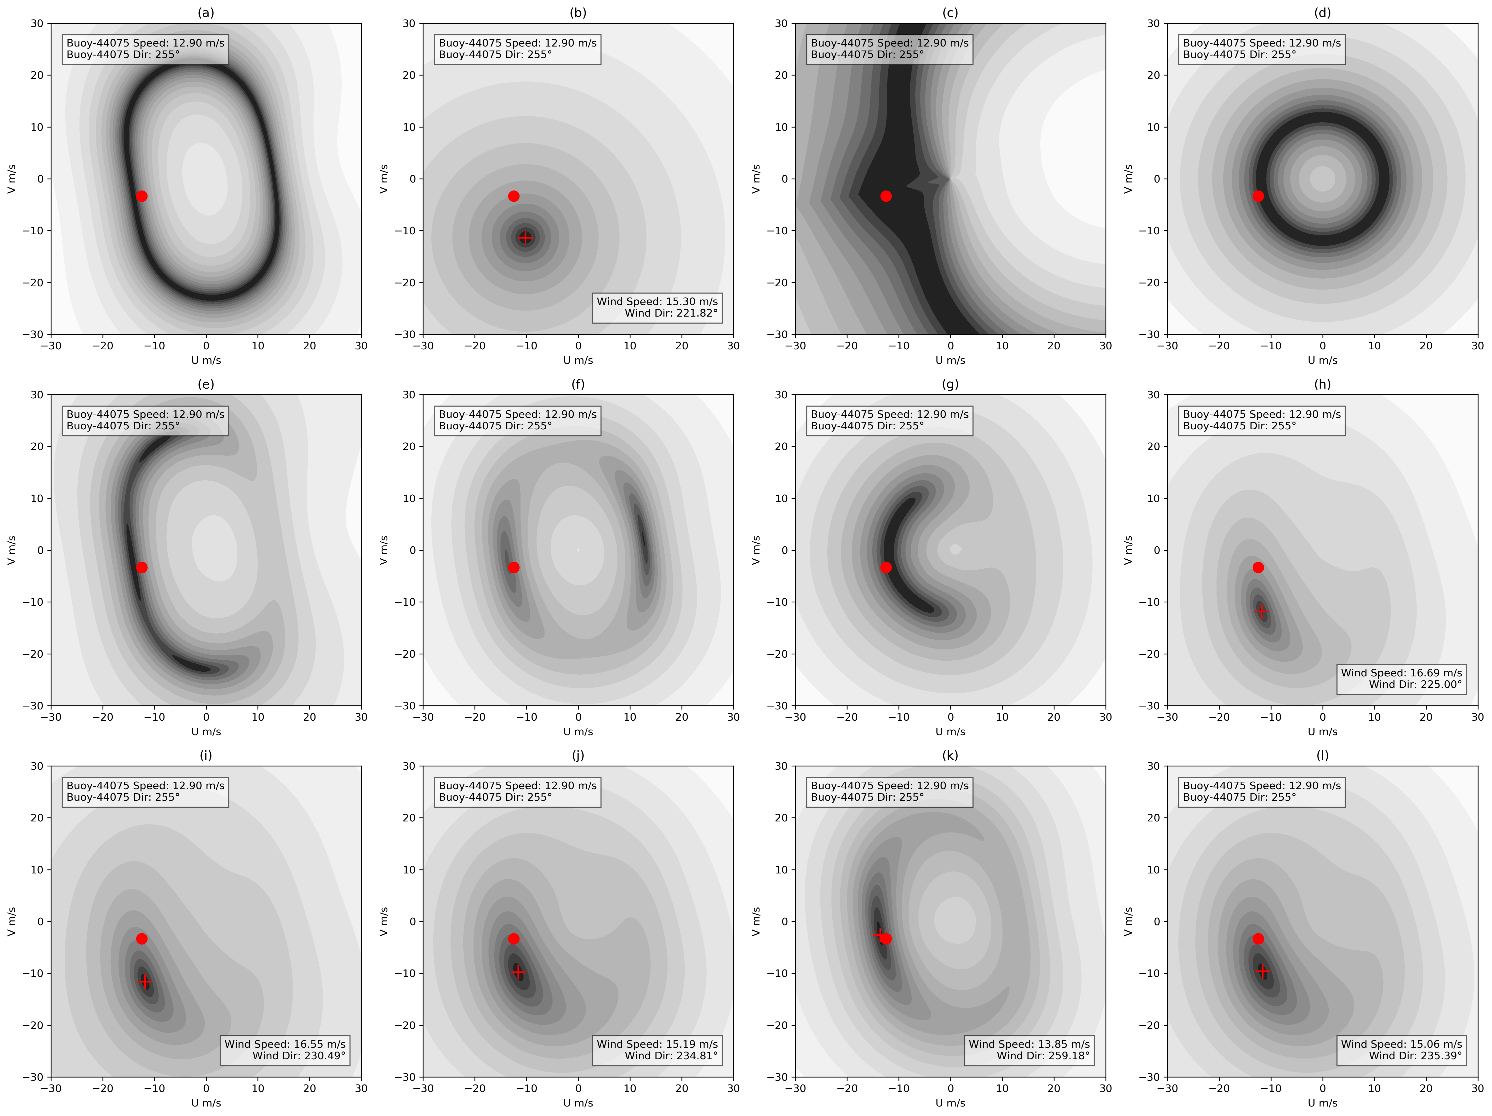
\includegraphics[width=.9\textwidth]{./figures/J}
	\caption{Cost function terms and their contributions. Darker shading indicates lower cost function values, representing a higher likelihood of the corresponding wind vector. Red circles denote the ``tru'' wind vector from buoy observations, while red crosses indicate the wind vector obtained by minimizing the cost function. Subfigures (a)-(d) show individual contributions of NRCS, background, Doppler, and azimuth wavelength cut-off terms. Subfigures (e)-(h) illustrate combined cost functions with, respectively, NRCS and Doppler, NRCS and azimuth wavelength cut-off, Doppler and azimuth wavelength cut-off terms, and NRCS and background, highlighting ambiguities. Subfigures (i)-(l) present inversion results for various term combinations: (i) corresponds to the combination of NRCS, Doppler and background, (j) that of NRCS. azimuth wavelength cut-off and background, (k) that of NRCS, Doppler and azimuth wavelength cut-off. Finally, (l) shows the combination of all terms in Equation \ref{eq: Bayes}.}
	\label{fig: J}
\end{figure}

Figure \ref{fig: J} shows a retrieval case study using a Sentinel-1 SAR image acquired on January 17, 2022, at 22:43:11 UTC over the Atlantic Ocean \cite{ZhuIGARSS2025}. As from the National Data Buoy Center (NDBC) buoy with ID 44075, wind speed and direction at 22:40 UTC measure 12.9 ms$^{-1}$ and 255$^{o}$, respectively, as also reported in the top-left corner of each subplot. The collocated ECMWF Re-analysis 5 (ERA5) wind speed and direction are 15.3 ms$^{-1}$ and 221.82$^{o}$, respectively. The buoy measurement and the background winds are represented with a red circle and a cross, respectively, in each plot. \\
Figure \ref{fig: J} shows the contribution of each term in Equation \ref{eq: Bayes} to the cost function (top row) and the contribution of their intersections two-to-two (central row) and three-to-three (first three plots of the bottom row). Finally, the plot in the bottom right corner shows the total cost function. Darker shading indicates lower cost function values, representing a higher likelihood of the corresponding wind vector. \\
Figure \ref{fig: J}a shows an elliptical symmetry, with the major axes tilted with respect to the north-south direction (v-axes). The inclination is due to the satellite platform's flying direction, which is ascending in this specific case. The along-track cross-track asymmetry is due to the bi-harmonic trend of CMOD7, as depicted in Equation \ref{eq: CMOD7}. Given the measured $\bar{\sigma}_{0}$, the NRCS term provides infinite solutions. This happens because a conventional SAR is a one-look instrument and has no azimuthal look diversity, useful to reduce the number of ambiguities, such as in scatterometers. \\
The background term has a sink shape, with the minimum in $\mathbf{u_{B}}$. Note that the ``true'' and background winds are not very close. This may happen in several situations, especially in rapidly changing weather patterns, such as fronts and extreme events, but also due to the ``phase shift'' of NWP models. Finally, the low spatial resolution of NWP models compared to SAR plays a non-negligible role \cite{VogelzangJGRO2011}. In these cases, the combination of the NRCS and background terms (Figure \ref{fig: J}h) can lead to high-biased solutions, as thoroughly discussed in \cite{PortabellaJGRO2002}. \\
The Doppler term (Figure \ref{fig: J}c) appears quite complementary to the NRCS term, and helps to reduce ambiguities, as shown in Figure \ref{fig: J}d. When combined with the background term (Figure \ref{fig: J}i), the a-posteriori pdf has a well-defined peak \cite{MoucheTGRS2012}. However, for the same reasons discussed before, this solution can be severely biased. \\
The azimuth wavelength cut-off term (Figure \ref{fig: J}d) shows a circular symmetry. This is in agreement with the model introduced in Equation \ref{eq: az cutoff}. Its combination with the NRCS term can help to reduce ambiguities, as shown in Figure \ref{fig: J}f, leading to a bi-modal a-posteriori pdf. However, this combination can be less fortunate, and the peaks of the a-posteriori pdf can be very spread, leading to a wide range of ambiguities. In other words, the synergy between the NRCS and azimuth wavelength cut-off terms is not optimal. Instead, when these terms are combined with the Doppler term, the solution converges towards the ``truth''. In this specific case study, this solution is even better than what is obtained when all terms are combined. Once more, this emphasizes the eventual biases of NWP. However, this is a fortunate case, which does not always happen. 

\subsection{Esample: SAR Significant Wave Height Retrieval}
\label{sec: SWH}

The retrieval algorithm discussed in this section is based on the linear relationship between the azimuth wavelength cut-off ($\lambda_{C}$) and the square root of the significant wave height ($H_{s}$), as described in Equation \ref{eq: lc vs hs} \cite{GriecoIJRS2016}:

\begin{equation}
	\lambda_{C} = b_{0}+b_{1}\sqrt(H_{s})
	\label{eq: lc vs hs}
\end{equation}

$H_{s}$ can be obtained by simply inverting Equation \ref{eq: lc vs hs}, which leads to Equation \ref{eq: hs}

\begin{equation}
	H_{s} = \left(\frac{\lambda_{C}-b_{0}}{b_{1}}\right)^{2}
	\label{eq: hs}
\end{equation}

The retrieval accuracy obtained with this algorithm is around 0.5 m \cite{GriecoIJRS2016}. \\
The error sources are described as follows:
\begin{itemize}
	\item $\epsilon(b_{i})$: uncertainty of the offset and slope estimates of Equation \ref{eq: lc vs hs};
	\item $\epsilon(\lambda_{C})$: uncertainty of $\lambda_{C}$ estimate;
\end{itemize}

Note that $\lambda_{C}$ is estimated through several steps. Starting from $\sigma_{0}$, all the steps are below:
\begin{itemize}
	\item Bright target removal. This step aims to remove bright spots that are supposed to be target echoes;
	\item Fast Fourier Transform (FFT) of the SAR sub-image of interest;
	\item Computation of cross-correlation spectrum (CCS);
	\item Range-averaging of CCS;
	\item Computation of the cross-correlation function (CCF) through inverse FFT of range-averaged CCS;
	\item Gaussian fit of CCF;
\end{itemize}

Each step is supposed to introduce additional error, which finally cumulate in $\epsilon(\lambda_{C})$.
Figure \ref{fig: SWH diag} shows the uncertainty \gls{traceability} diagram.

\begin{figure}[h]
	\centering
	\newcommand\ys{1.cm}
	\newcommand\xs{2.cm}
	%\fontsize{8}{9}\selectfont
	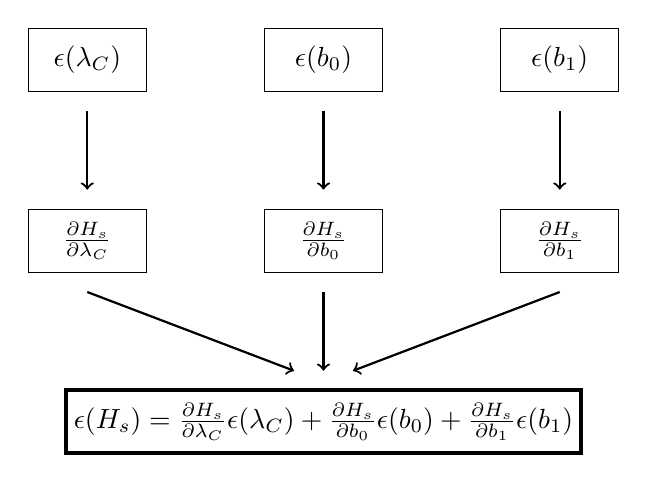
\begin{tikzpicture}[myarrow/.style={single arrow,single arrow head extend=.1cm,anchor=west,minimum height=.8cm,minimum width=.1cm},
		myrectangle/.style={rectangle,draw=black,text=black,inner sep=.1cm, outer sep=.25cm, minimum width=1.5cm, minimum height=.8cm}],
		\node(eH)[myrectangle,line width=.5mm,align=center,anchor=east] at (0.cm, 0.cm) 
		{$\epsilon(H_{s})=\frac{\partial H_{s}}{\partial \lambda_{C}}\epsilon(\lambda_{C})+\frac{\partial H_{s}}{\partial b_{0}}\epsilon(b_{0})+\frac{\partial H_{s}}{\partial b_{1}}\epsilon(b_{1})$};
		\node(dHdl)[myrectangle,align=center,anchor=south] at ([xshift=-1.5*\xs,yshift=\ys]eH.north) {$\frac{\partial H_{s}}{\partial \lambda_{C}}$};
		\node(el)[myrectangle,align=center,anchor=south] at ([yshift=\ys]dHdl.north) {$\epsilon(\lambda_{C})$};
		\node(dHda)[myrectangle,align=center,anchor=south] at ([yshift=\ys]eH.north) {$\frac{\partial H_{s}}{\partial b_{0}}$};
		\node(ea)[myrectangle,align=center,anchor=south] at ([yshift=\ys]dHda.north) {$\epsilon(b_{0})$};
		\node(dHdb)[myrectangle,align=center,anchor=south] at ([xshift=1.5*\xs,yshift=\ys]eH.north) {$\frac{\partial H_{s}}{\partial b_{1}}$};
		\node(eb)[myrectangle,align=center,anchor=south] at ([yshift=\ys]dHdb.north) {$\epsilon(b_{1})$};
		\path [black, thick, ->] (dHdl.270) edge node {} (eH.120);
		\path [black, thick, ->] (dHda.270) edge node {} (eH.90);
		\path [black, thick, ->] (dHdb.270) edge node {} (eH.60);
		\path [black, thick, ->] (el.270) edge node {} (dHdl.90);
		\path [black, thick, ->] (ea.270) edge node {} (dHda.90);
		\path [black, thick, ->] (eb.270) edge node {} (dHdb.90);
	\end{tikzpicture}
        \caption{Uncertainty Traceability Diagram for the significant wave height retrieval algorithm presented.}
	\label{fig: SWH diag}
\end{figure}

Demonstrate identification, modeling and propagation of uncertainties.

%\subsection{Example: Wet Snow Retrieval}
%
%Demonstrate identification, modeling and propagation of uncertainties.
%
%\subsection{Example: Soil Moisture}
%
%Demonstrate identification, modeling and propagation of uncertainties.
%
%\subsection{Example: Sea State}

